\documentclass[conference]{IEEEtran}

\IEEEoverridecommandlockouts
\usepackage{cite}
\usepackage[justification=centering]{caption}
\usepackage{amsmath,amssymb,amsfonts}
\usepackage{algorithmic}
\usepackage{graphicx}
\usepackage{textcomp}
\usepackage{xcolor}
	
\begin{document}

\title{
	Simultaneous Localization and Monitoring \\ with Gaussian Processes \\
}

\author {
	\IEEEauthorblockN{B. Sc. Oliver Neumann}
	\IEEEauthorblockA {
		\textit{Computer Science Student} \\
		\textit{Karlsruher Institut of Technology (KIT)}\\
		%Karlsruhe, Germany \\
		%email address
	} \and
	\IEEEauthorblockN{Dipl. Phys. Jana Mayer}
	\IEEEauthorblockA {
		\textit{Intelligent Sensor-Actor-Systems (ISAS)} \\
		\textit{Institute for Anthropomatics} \\
		\textit{and Robotics (IAR)} \\
		%Karlsruhe, Germany \\
		%email address
	} \and
	\IEEEauthorblockN{Dr. Ing. Benjamin Noack}
	\IEEEauthorblockA {
		\textit{Intelligent Sensor-Actor-Systems (ISAS)} \\
		\textit{Institute for Anthropomatics} \\
		\textit{and Robotics (IAR)} \\
		%Karlsruhe, Germany \\
		%email address
	}
}

\maketitle

\begin{abstract}
    Simultaneous localization and mapping (SLAM) became one of the most important
    research fields in the last two decades. There are also recent approaches
    facing SLAM with the use of physical phenomena. That is a promising step
    for many use cases, like indoor navigation. One challenging part of those
    approaches is to switch from discrete landmarks to continuous functions.
    This function often needs to be approximated for SLAM and also for monitoring
    usages. In this paper the basic knowledge of SLAM is explained and the mathematics
    behind gaussian processes is introduced. Moreover, recent approaches facing
    SLAM in combination of monitoring, using physical phenomena for SLAM in real time
    and modeling uncertainty in the input of gaussian processes, will be presented.
    At the end, open questions which could be faced in further proceeding are discussed.
\end{abstract}

%\begin{IEEEkeywords}
%    SLAM, monitoring, physical phenomenon, gaussian process
%\end{IEEEkeywords}

\section{Introduction}
\subsection{Motivation}
Robots often have to move in an unknown environment. For that, a robot has to build up a map
and locate itself in this environment. This kind of problem became a large research
field in the last two decades under the name of \textit{Simultaneous Localization and Mapping
(SLAM)}. Most techniques use landmarks seen by a camera. The robot tries
to see the landmarks in two successive images again and estimate its new position by the change
of the landmarks. Figure \ref{fig:grisetti_slam_example} is showing landmarks on the floor prepared 
for the robot so it can use SLAM. But preparation isn't needed every time, higher-priced vacuum cleaning 
robots for example using SLAM with a camera looking at the ceiling.

\begin{figure}[h!]
	\centering
	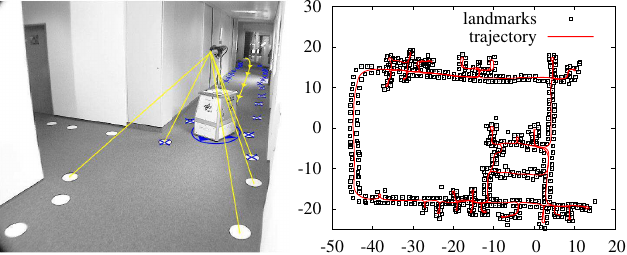
\includegraphics[width=0.5\textwidth]{images/grisetti_slam_example.png}
	\caption{
		An illustration for SLAM with prepared environment for the robot.
		Landmarks are mounted on the floor which the robot can recognize (left image).
		The generated map is shown on the right \cite{grisetti_tutorial_2010}.
		}
	\label{fig:grisetti_slam_example}
\end{figure}

Recent researchers are trying to use physical phenomena instead of landmarks with promising results. 
For example wifi signal or the magnetic field. This opens a completely new variety of possible applications. 
Environments where landmarks of a camera are not suitable for SLAM applications like underwater. Also, scenarios 
where monitoring of a physical phenomenon is the aim and this phenomenon is also suitable for SLAM. So, there
is no need for extra equipment mounted on the robot which saves money.

However, switching from landmarks to physical phenomena is not trivial. The main difference is that landmarks
are discrete in space and physical phenomena are continuous and there can't be made any assumptions to the
underlying function (e.g. it can be described by a polynomial). Moreover, a moving robot will see different
landmarks multiple times and can set its position in relation to it. In case of physical phenomena,
there are only measurements possible at the current position of the robot which is uncertain. But every 
measurements are correlating which can be used to estimate a position or trajectory of the robot. This 
correlation is modeled within the covariance matrix of a gaussian process which will be discussed in 
\ref{chap:gaussian}.

\subsection{State of the art SLAM}
\label{chap:slam}
As mentioned before, SLAM describes the field of problem where an agent or robot has to locate itself
in an unknown environment. Therefore the agent has to build up a map. The map normally containing discrete 
landmarks but also continuous functions or planes (as an approximation of the world) could be possible. 
All of the techniques have in common, that the created map is always an estimation. So SLAM is a 
probabilistic approach. The reason for that is, that all data given is uncertain. Such as current 
position, measured value (e.g. magnetic field) or landmark position. The noise of the measurements is 
normally gaussian distributed. 

When thinking of SLAM there are two common classifications \cite{grisetti_tutorial_2010}. The first 
class models SLAM as an on-line state estimator, where the state is the current position of the robot 
within the map. This approach is called filtering or on-line SLAM. In contrast to that smoothing 
approaches attempt to estimate the full trajectory of the robot based on all measurements. 
Often smoothing is called full SLAM.

Regardless of filtering or smoothing approaches, they often using Kalman or particle filter to estimate
the current state \cite{grisetti_tutorial_2010}. Kalman filter is a mathematical concept and is also known
as linear quadratic estimation (LQE). It contains two major steps, prediction and update.
In the prediction step the next state is predicted by using the currently given data. After that, 
the prediction will be improved by combining the estimated state from the prediction with the new 
measured state \cite{kalman_filter_2001}. This step is called update. Kalman filter always follow only one
hypothesis. In contrast to that particle filters where invented. Each particle follows a specific
hypothesis and normally there are multiple particles. So, particle filter follow multiple hypothesis.

\begin{figure}[h!]
	\centering
	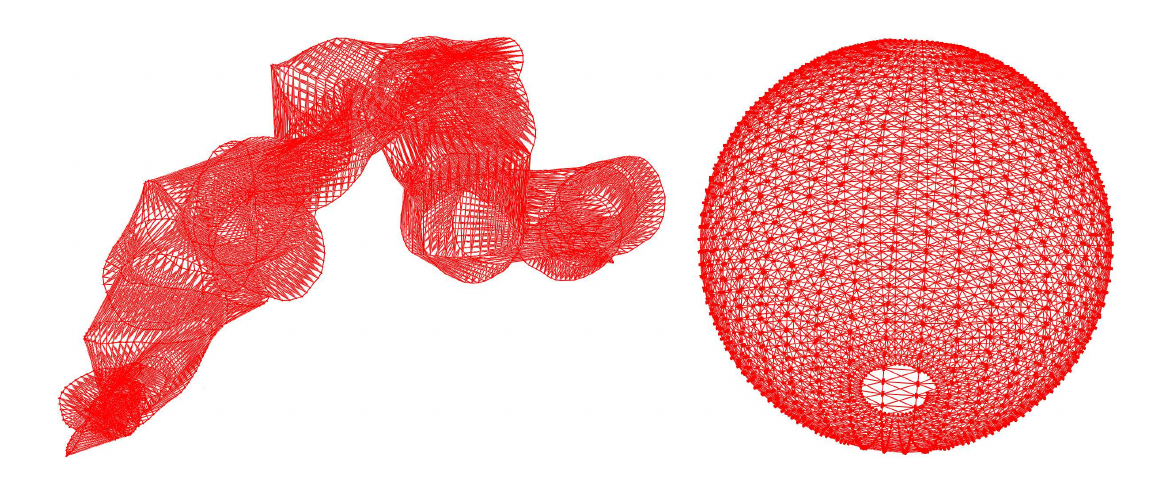
\includegraphics[width=0.5\textwidth]{images/grisetti_slam_showcase.png}
	\caption{
        Showcase of a current state-of-the-art graph-based SLAM approach.
        Initial position estimation on the left and next to it graph-based 
        SLAM position estimation. The robot was moved in a simulation on 
        the surface of a sphere \cite{grisetti_tutorial_2010}.
        }
	\label{fig:grisetti_slam_showcase}
\end{figure}

Current state-of-the-art techniques of SLAM using graph-based approaches. A performance showcase of 
that is shown in figure \ref{fig:grisetti_slam_showcase}. The idea of those approaches is easy to 
understand. While the robot is moving and making measurements a graph is build up as illustrated in 
figure \ref{fig:kaess_slam_graph}. With graph algorithms the positions $x_0$, ..., $x_n$ can now be
estimated.

\begin{figure}[h!]
	\centering
	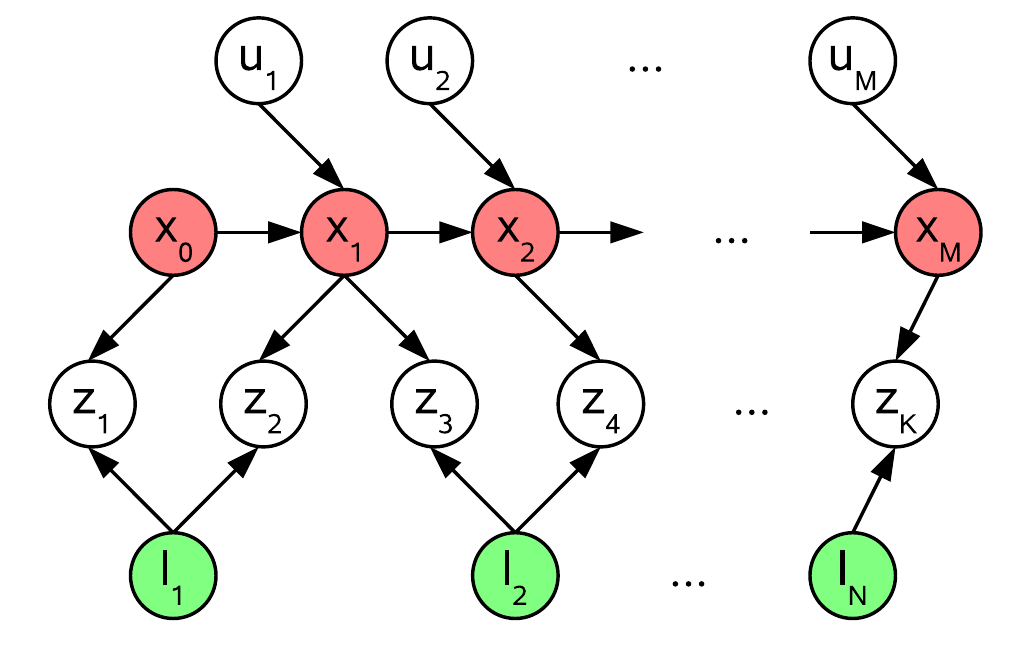
\includegraphics[width=0.45\textwidth]{images/kaess_slam_graph.png}
	\caption{
        SLAM graph with $x_i$ as the robot position at time step $i$. $l_j$ is the $j^{th}$ landmark. 
        $z_k$ is the $k^{th}$ by the robot measured landmark. $u_i$ is the control input at time step 
        $i$ which is for example odometry data \cite{kaess_isam:_2008}. For understanding: 
        At time step $1$ the robot position was $x_1$ and it measured landmark $l_1$ and $l_2$ 
        which can be seen by the measurements $z_2$ and $z_3$. The input from the control unit was $u_1$.
        }
	\label{fig:kaess_slam_graph}
\end{figure}

\subsection{Gaussian Process}
\label{chap:gaussian}
In case of SLAM with physical phenomena, the approximation of the underlying function can be done 
with Gaussian processes. A Gaussian process is a stochastic process, so it consists of a set of random
variables which are index by time or space. Random variables of a Gaussian process are especially multivariate
normally distributed. So every finite subset of a Gaussian process is again multivariate normally distributed.

Gaussian processes are defined by a mean function $m(t)$ and a covariance function $k(x_i, x_j)$ also called kernel.
If $m(t) = 0$ the Gaussian process is called centered. For the kernel, radial basis function can be used. Such
Gaussian processes are called radial. For a radial covariance function follows $k(x_i, x_j) = k(||x_i - x_j||)$. 
One very common radial kernel is the squared exponential kernel \cite{ebden_gaussian_2015}

$$
k(x_i, x_j) = \sigma ^2 \exp 
\begin{pmatrix}
	-\frac{(x_i - x_j)^2}{2l^2}
\end{pmatrix}\text{.}
$$

It is also possible to model noisy measurements with Gaussian processes. Assume the noise is normal distributed
with variance $\sigma^2$. Then measurements can be described like $y_i = f(x_i) + \mathcal{N}(0, \sigma^2)$.
Combining the covariance function with the model of noisy measurements, that will lead to the slightly 
changed kernel
$$
k(x_i, x_j) = \sigma ^2 \exp 
\begin{pmatrix}
	-\frac{(x_i - x_j)^2}{2l^2}
\end{pmatrix}
+ \delta_{ij} \sigma^2_{noise}\text{ .}
$$
In this kernel $\delta_{ij}$ is the Kronecker delta. This function is only $1$ when $i=j$ otherwise it is $0$. 
So, $\sigma^2_{noise}$ is only added to the measurements. Figure \ref{fig:gaussian_process_example} gives an example 
for Gaussian processes with and without noisy measurements.

Assume now there are $n$ measurements $y_1, ..., y_n$ taken at $x_1, ..., x_n$. Then the covariance matrix 
would be
$$
K = \begin{bmatrix}
	k(x_1, x_1) & k(x_1, x_2) & \dots & k(x_1, x_n) \\
	k(x_2, x_1) & k(x_2, x_2) & \dots & k(x_2, x_n) \\
	\vdots & \vdots & \ddots & \vdots \\
	k(x_n, x_1) & k(x_n, x_2) & \dots & k(x_n, x_n) \\
\end{bmatrix}\text{.}
$$
Estimating $y^*$ at $x^*$ and assuming the kernel is radial, would lead to a covariance matrix
$$
\begin{bmatrix}
	K & K_*^T \\
	K_* & K_{**} \\
\end{bmatrix} \text{ with}
$$
$$
K_* = [k(x_*, x_1), \dots, k(x_*, x_n)],
$$
$$
K_{**} = k(x_*, x_*)\text{.}
$$
Because of Gaussian processes modeling data from a multivariate normal distribution, $y$ and $y_*$ 
can be modeled as
$$
\begin{bmatrix}
	y \\
	y_* \\
\end{bmatrix} 
\sim
\mathcal{N} 
\begin{pmatrix}
	0, 
	\begin{bmatrix}
		K & K_*^T \\
		K_* & K_{**} \\
	\end{bmatrix}
\end{pmatrix}\text{.}
$$
Using the mathematics of multivariate Gaussian distributions, the most likely value of $y_*$ can be 
calculated by
\newpage
$$
y_*|y \sim \mathcal{N}(K_*K^{-1}y, K_{**} - K_*K^{-1}K_*^T)
$$
$$
\Rightarrow \bar{y}_* = K_*K^{-1}y\text{ .}
$$
The derivation of the formula is well explained by Ebden, 2008 \cite{ebden_gaussian_2015}. Notice that
also the variance for $y_*$ is given by
$$
var(y_*) = K_{**} - K_*K^{-1}K_*^T\text{ .}
$$

All that, uncertainty in measurements, prediction of $y_*$ and probability of the prediction can be seen
in Figure \ref{fig:gaussian_process_example}. Note that for linear increasing number of measurements the 
size of the covariance matrix rises quadratically and for $y_*$ the inverse of that matrix has to be calculated. 
So it is computational expensive for large-scale data. Some approaches facing that will be described in the 
next chapter. Another remark is that the standard Gaussian process is not possible to model uncertainty in the 
input data. A recent approach for that will also be presented in the Chapter \ref{chap:uncertain_inputs}. 

\begin{figure}[h!]
	\centering
	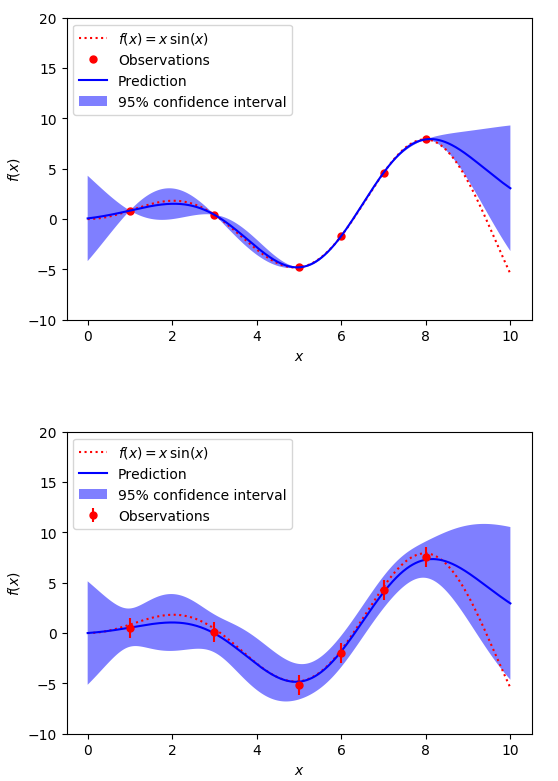
\includegraphics[width=0.425\textwidth]{images/gaussian_process_example.png}
	\caption{
			Plot of two Gaussian processes regressions with the same measurement points $x_i$
			but the one at the bottom has noisy measurements with variance $\sigma_{noise}^2 = 1$.
			Also noticeable the probability of the predictions represented through the confidence interval.
        }
	\label{fig:gaussian_process_example}
\end{figure}



\section{Current Work}
This chapter will present some recent scientific work. Aim is to give an overview
of the current work done in context of SLAM with monitoring, SLAM with physical phenomena and 
gaussian processes. 

\subsection{Monitoring with Complete Coverage}
\label{chap:complete_coverage}
Wieser and his team of researches faced the problem of monitoring an indoor magnetic field with high
spatial resolution \cite{wieser_slam_indoor_2014}. They don't use the magnetic field for
SLAM instead they use a camera mounted on top of the mobile robot. For the configuration space
a grid based representation is used. On this configuration space graph search algorithms, like 
Best-First-Search and Dijkstra, where applied to find the best way through the environment with
complete coverage \cite{wieser_slam_indoor_2014}. Figure \ref{fig:wieser_result} shows
the final result. Wieser et al. do not use any kind of regression to approximate the magnetic field.

\begin{figure}[h!]
	\centering
	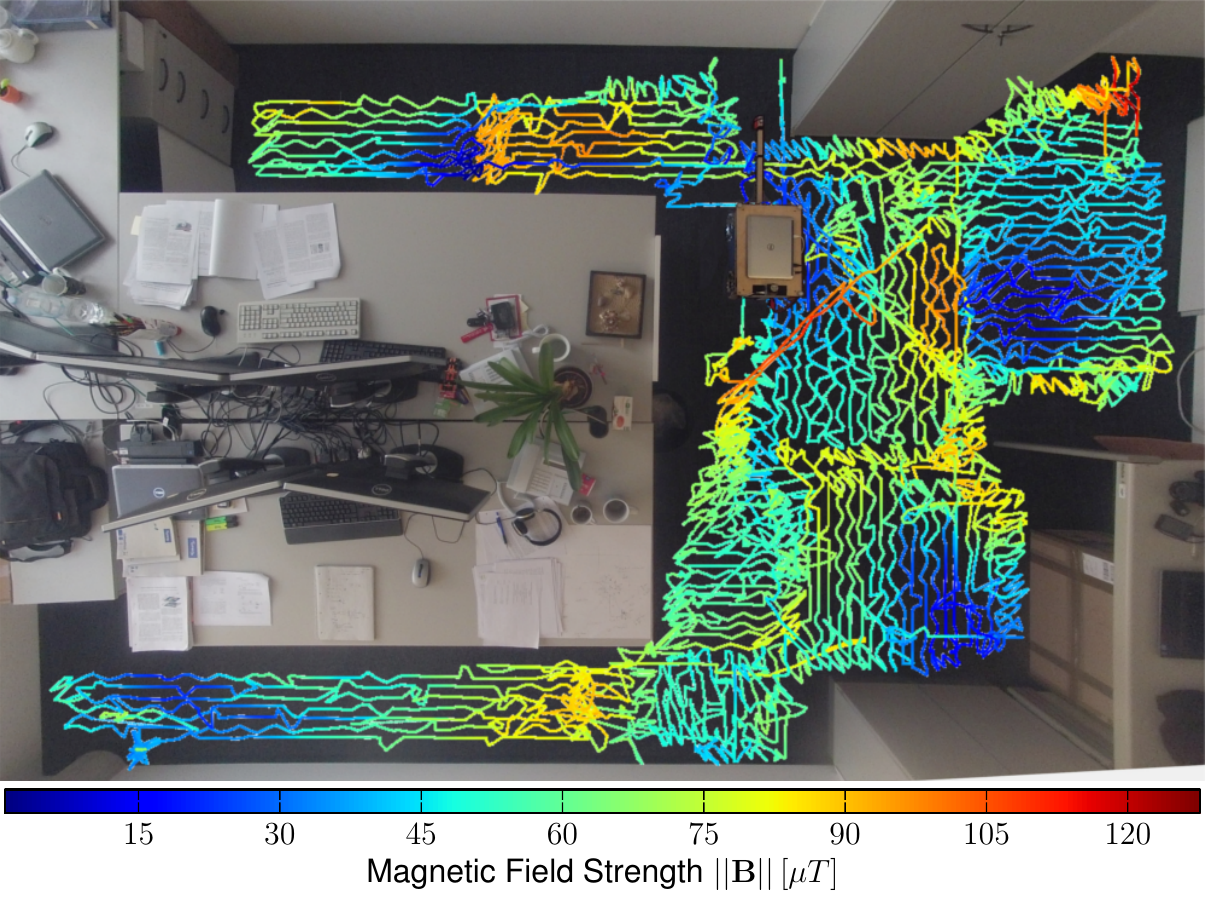
\includegraphics[width=0.45\textwidth]{images/wieser_result.png}
	\caption{
            Final result of Wieser et al. \cite{wieser_slam_indoor_2014}. It shows
            the complete coverage trajectory with measurements of the magnetic 
            field. The robot went through the office and the
            measurements have a spatial resolution of 0.05m \cite{wieser_slam_indoor_2014}.
        }
	\label{fig:wieser_result}
\end{figure}

Their program consists of four different threads. One thread processes the images by the camera
for localization and mapping and writes its result into a workspace. A thread called configuration
space mapper, processes data from the workspace and gathering data from the magnetic field sensor.
The result of that process is written into a configuration space. A path planning thread uses this
information to plan an optimal way. The last thread is called robot controller and has to perform 
the path given by the path planner while controlling the actuators of the robot. An illustration of 
that system can be seen in figure \ref{fig:wieser_system}.

\begin{figure}[h!]
	\centering
	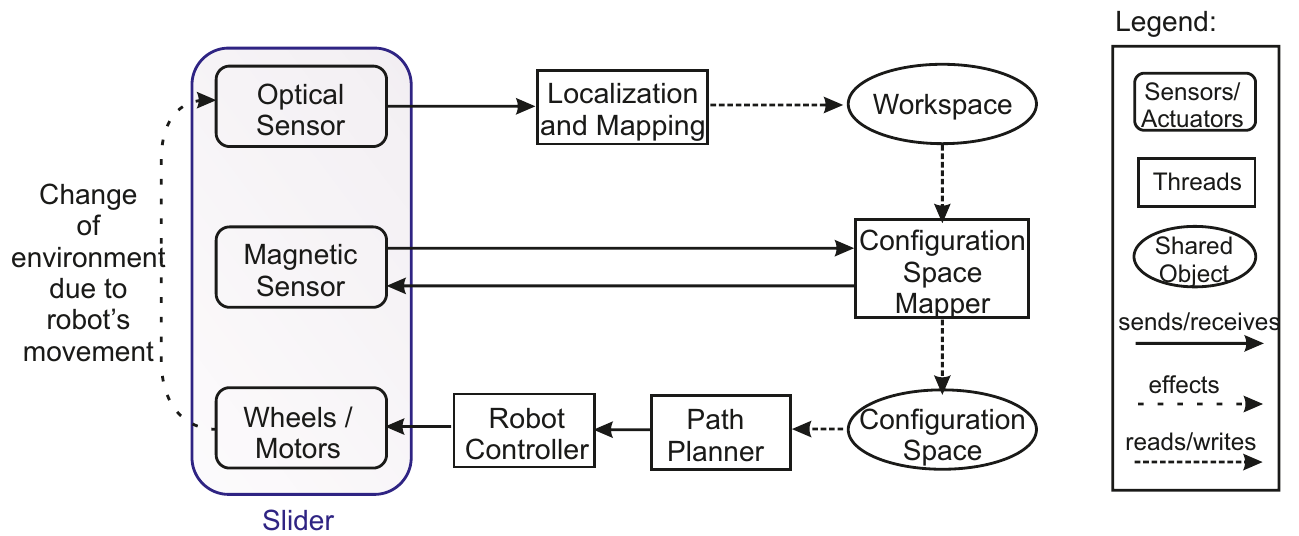
\includegraphics[width=0.5\textwidth]{images/wieser_system.png}
	\caption{
            System diagram shows the basic functionality of the approach by wieser et al. 
            \cite{wieser_slam_indoor_2014}.
        }
	\label{fig:wieser_system}
\end{figure}

\subsection{Scalable Magnetic Field SLAM}
Manon Kok and Arno Solin present in their paper an approach for scalable on-line SLAM in 3D using
magnetic field and gaussian processes \cite{kok_scalable_2018}. An example is shown
in figure \ref{fig:kok_3d}. In their work they had to face some problems which are already mentioned 
before. Approximate the underlying function of the magnetic field with gaussian processes. Handle 
large scale data because of on-line requirements. Using physical phenomena instead of images for 
SLAM approaches.

\begin{figure}[h!]
	\centering
	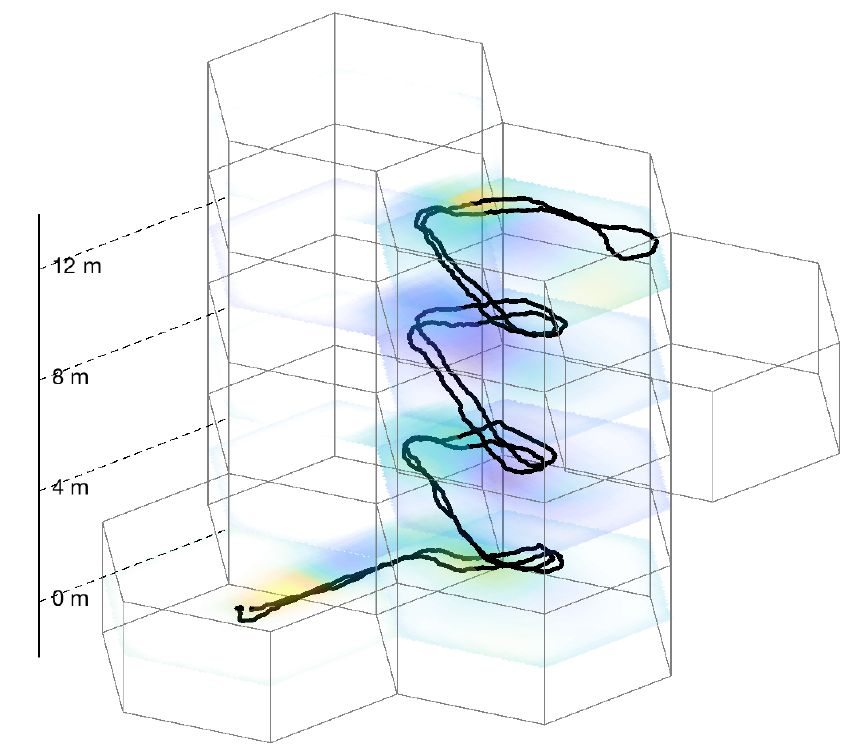
\includegraphics[width=0.45\textwidth]{images/kok_3d.png}
	\caption{
        Example by Manon Kon and Arno Solin showing 3D SLAM using magnetic field.
        The dataset was recorded at the University of Cambridge at the stairs of
        the Engineering Department \cite{kok_scalable_2018}.
        }
	\label{fig:kok_3d}
\end{figure}

To approximate the magnetic field, they use a combination of two kernels, the linear and squared
exponential kernel and a mean centered around zero \cite{kok_scalable_2018}. That leads to the 
following gaussian process.
$$
GP(0, k_{lin}(x_i, x_j) + k_{se}(x_i, x_j)) \text{ with}
$$
$$
k_{lin}(x_i, x_j) = \sigma_{lin}^2 x_i^T x_j, 
$$
$$
k_{se} = \sigma_{se}^2 \exp 
\begin{pmatrix}
    -\frac{||x_i - x_j||^2}{2l^2}
\end{pmatrix}
$$

To face the problem of on-line requirements, they divided the 3D space into hexagonal blocks
(See Figure \ref{fig:kok_3d} and \ref{fig:kok_example}). For each block there is a gaussian 
process for all data points within this block. This makes the covariance matrix for a block
much smaller than one large one. Every time a measurement is taken at a position where no hexagonal 
block exists, a new block will be created. Through that approach it is possible to do SLAM on the 
magnetic field in real time. A demonstration for that is given by them in a video they produced 
\cite{kok_scalable_2018}.

\begin{figure}[h!]
	\centering
	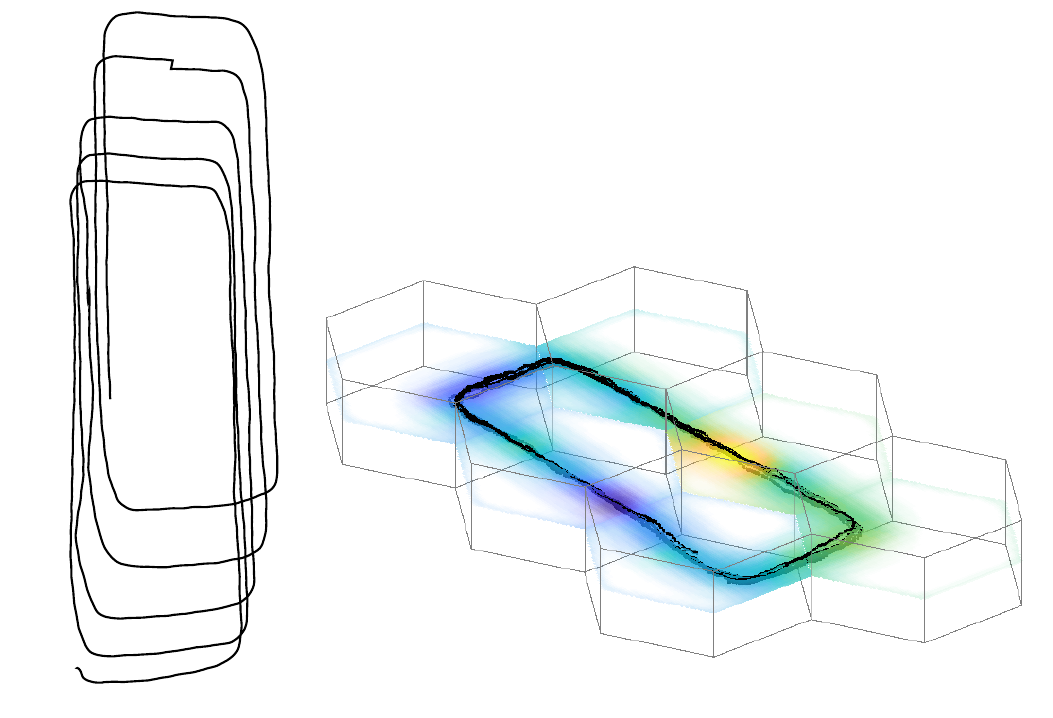
\includegraphics[width=0.5\textwidth]{images/kok_example.png}
	\caption{
        Performance demonstration of the SLAM algorithm by Kok and Solin \cite{kok_scalable_2018}.
        The trajectory on the left shows the odometrie data collected by a iPhone 6s and next to it
        the resulting trajectory with the approximated magnetic field.
        }
	\label{fig:kok_example}
\end{figure}

As mentioned in chapter \ref{chap:slam} current state of the art approaches of SLAM using graph-based
techniques. Kok and Solin don't use a graph-based approach. They choose a combination of Kalman
and particle filtering. The Kalman filter is used for update measurements and the particle filter
for predictions in time. For more information, a description of the algorithm can be found in their
paper \cite{kok_scalable_2018}. A performance demonstration is shown in figure \ref{fig:kok_example}.

\subsection{Terrain Field SLAM}
\label{chap:terrain_field}
One interesting approach from Hyeonwoo Yu and Beomhee Lee deals with terrain field SLAM \cite{yu_terrain_2018}. 
They used the vibrations obtained from the robot, which are caused by the interaction between the terrain and 
the mobile robot, as the physical phenomenon for SLAM. Their experimental setup containing the robot and an
area with different subsurfaces which can be seen in figure \ref{fig:yu_setup}.

\begin{figure}[h!]
	\centering
	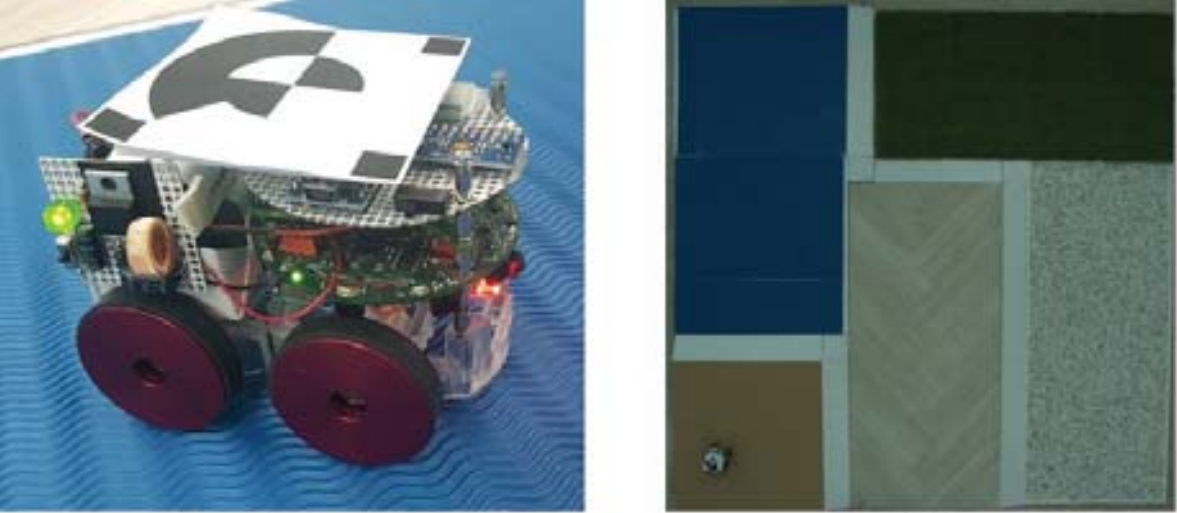
\includegraphics[width=0.5\textwidth]{images/yu_setup.png}
	\caption{
        Illustration of the setup by Yu and Lee. The mobile robot at the left and
        on the right the environment for the robot to move in. The environment containing
        five different subsurfaces \cite{yu_terrain_2018}.
        }
	\label{fig:yu_setup}
\end{figure}

Also, Yu and Lee used gaussian processes to infer the terrain field. Although, they don't face the
problem of doing SLAM and gaussian process regression on-line. A performance example of their approach
is shown in figure \ref{fig:yu_performance}. There is a little derivation over time, but
for the given terrain field the result is considerable \cite{yu_terrain_2018}.

\begin{figure}[h!]
	\centering
	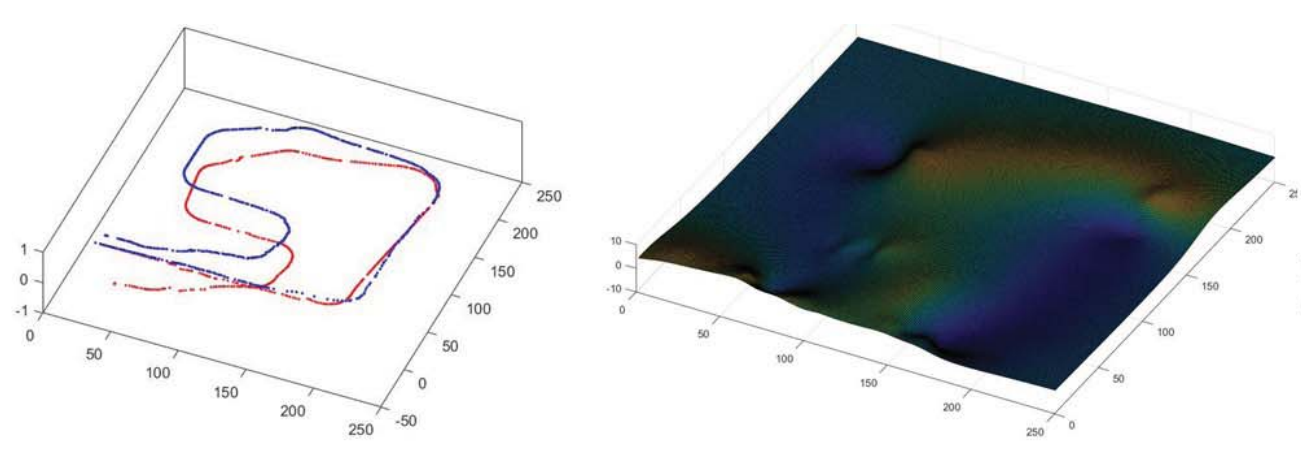
\includegraphics[width=0.5\textwidth]{images/yu_performance.png}
	\caption{
        Performance illustration of the terrain based SLAM approach by Yu and Lee \cite{yu_terrain_2018}.
        Robot trajectory in red on the left and ground truth in blue. On the right inferred terrain field.
        }
	\label{fig:yu_performance}
\end{figure}

\subsection{Uncertain Inputs with Gaussian Processes}
\label{chap:uncertain_inputs}
As mentioned in chapter \ref{chap:gaussian} uncertain inputs are not a part of standard gaussian processes
\cite{damianou_variational_2014}. So researchers have to face that problem. One team which did that is 
Andreas C. Damianou et al. First they modeled the uncertain input as:
$$
z_i \sim \mathcal{N}(x_i, \sigma_{noise})
$$
Which leads to a gaussian prior distribution over $X$:
$$
p(X|Z) = \prod_{i=1}^{\infty} \mathcal{N}(x_i| z_i, \sigma_{noise})
$$
That prior distribution they combining with the gaussian process latent variable model to handle
uncertain inputs. As an example they propagating frames in videos. For that they choose a 
fix windows size and use the frames as input for forecasting new frames. Although, frames
of the video don't have to be noisy the propagated frames are. This propagated frames are the input 
for the next time steps and because they were forecasted they are uncertain. With gaussian processes 
it is also possible to calculate the uncertainty and variance of the propagated frames which is useful 
for handling uncertain input. An example is shown in figure \ref{fig:damianou_example}.

\begin{figure}[h!]
	\centering
	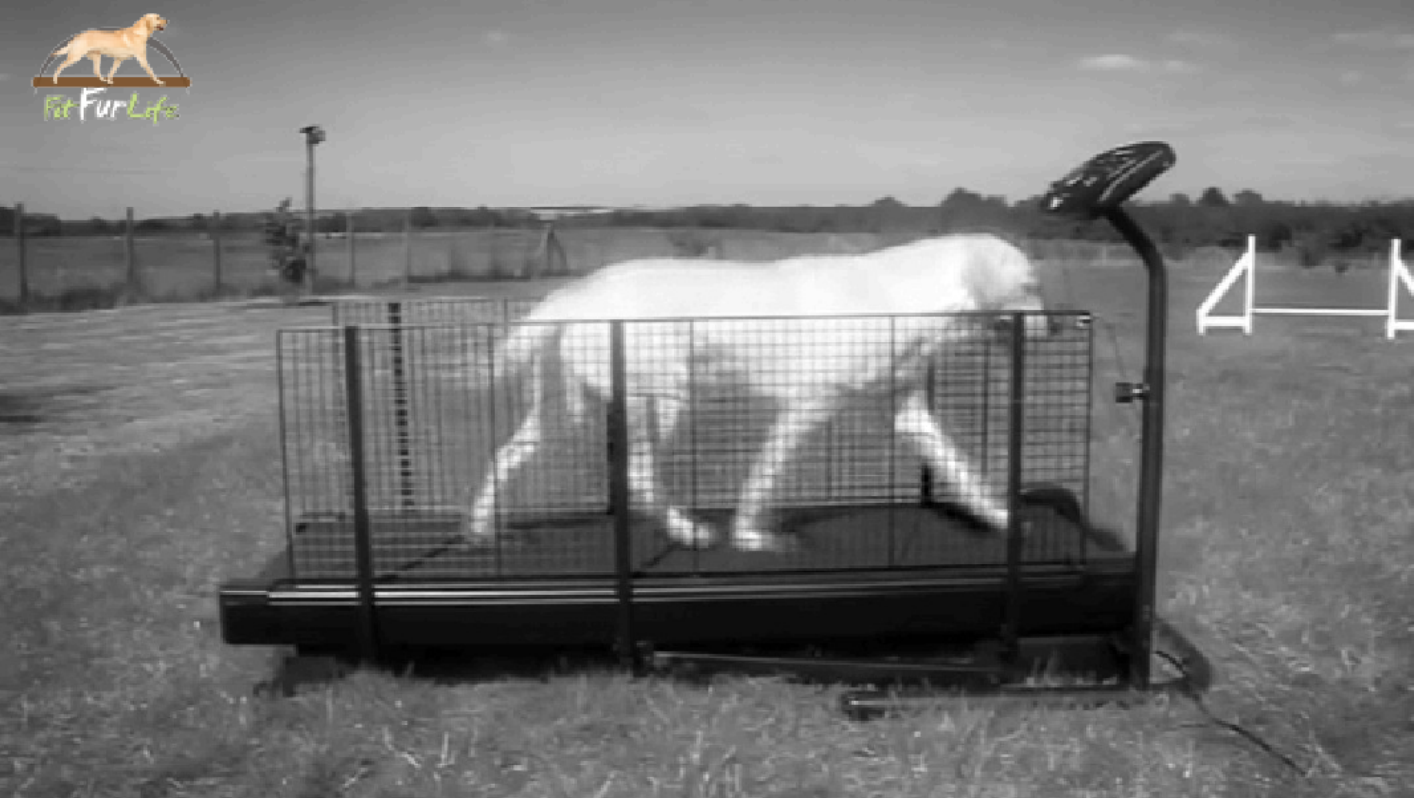
\includegraphics[width=0.425\textwidth]{images/damianou_example_1.png}
	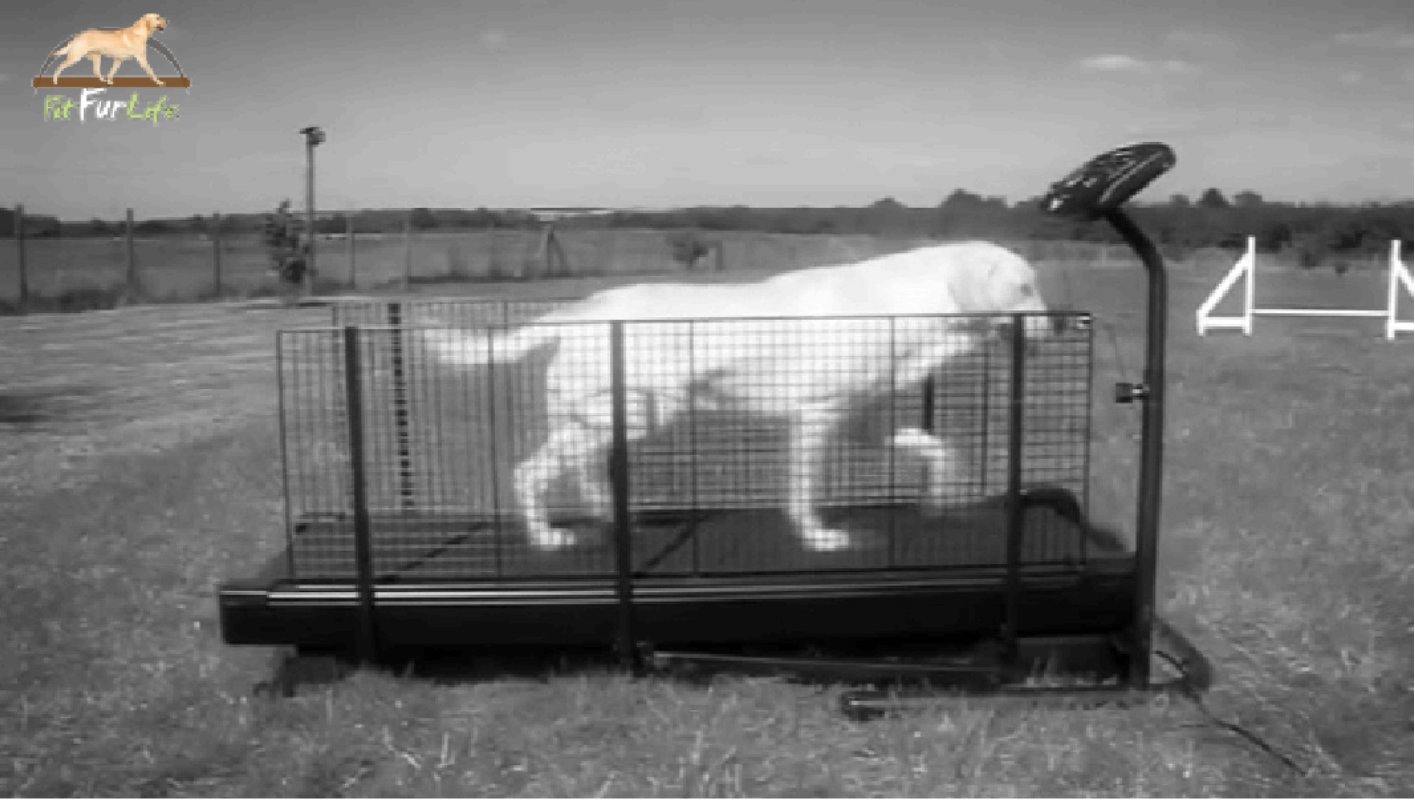
\includegraphics[width=0.425\textwidth]{images/damianou_example_2.png}
	\caption{
		Propagation demonstration of video frames. Top image shows an example
		frame of the input window for propagating the next frame (bottom). 
        }
	\label{fig:damianou_example}
\end{figure}

\section{Conclusion}
When facing the problem of SLAM using physical phenomena one challenge is
to handle continuous functions in contrast to discrete landmarks. Moreover,
the physical phenomena need to be approximated to use in case of SLAM. 
For that, gaussian processes are needed.

In chapter \ref{chap:slam} a current state-of-the-art graph-based SLAM
techniques is discussed. This approach is proven but it's only working
in case of landmarks. It should be possible to formulate the problem
of SLAM using physical phenomena in a graph-based manner. This could
be faced in later proceedings.

A terrain field based SLAM approach was discussed in \ref{chap:terrain_field}.
It showed that a variety of phyiscal phenomena could be used for a SLAM approach.
In further studies different phenomena could be observed and analyzed how suitable
they are for SLAM approaches. E.g. texture of a subsurface measured by a camera,
emission in a city or environmental sound.

Thinking of different suitable phyiscal phenomena would also lead to the question
how to handle phenomena which change in time. Imagine autonomous submarine using
sea streams for SLAM to monitor a gas pipeline. But sea streams won't be stable
in time. How to still use sea streams for SLAM also would need more research to do.

Another interesting thought is using only gaussian processes with uncertain input
for SLAM without any common SLAM techniques like Kalman filter or graph-based 
approaches. The idea would be that all measurements are taken at an uncertain
position which is the input for the gaussian process. To use gaussian processes
for that case, the uncertainty in the input has to decrease. Current researchers
often only face the problem of getting more accurate in the output but not in the
input data. Equally like the presented paper from Damianou et al. in chapter 
\ref{chap:uncertain_inputs}.

As mentioned before, different phenomena could be used for SLAM. Also, it could 
be an aim to monitor that phenomena. But when it comes to combining monitoring
and SLAM there has to be more work to do. In \ref{chap:complete_coverage} a
traditional SLAM approach with focus on monitoring was introduced, but how to
deal with phenomena changing over time (so they need to be monitored)? The certainty 
in the measurements should decrease over time, because the measurements getting older. 
So, there are also questions to answer.

In conclusion, there are many different problems to solve. Thinking of combining
SLAM with physical phenomena and the aim of monitoring these. Also, getting away
from traditional SLAM approaches and only using gaussian processes with uncertain
input or just consider new suitable physical phenomena for SLAM as mentioned before.

\nocite{*}

\bibliography{sources}{}
\bibliographystyle{ieeetr}

\end{document}
